\section{Case-studies} \label{sec:results}

Following case-studies test and assess the output of some of the real life sheet metal parts.


\def\finalcolumn{0.245} 

\begin{figure}[!h]
\centering     
\subfloat[Original Model]{\label{fig:results:originalenclosurepart}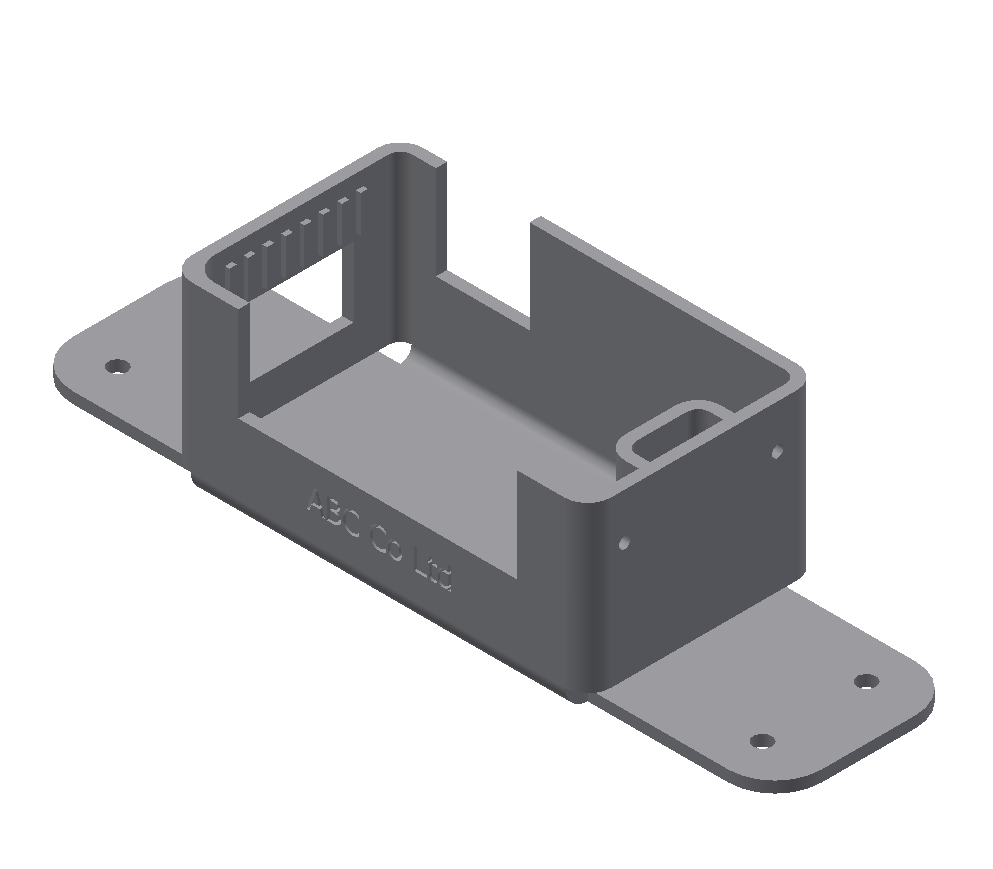
\includegraphics[width=\finalcolumn\linewidth,valign=t]{../Common/images/SheetMetal_Medium_Enclosure_OriginalPart}} 
\subfloat[Model Simplification]{\label{fig:results:defeaturing}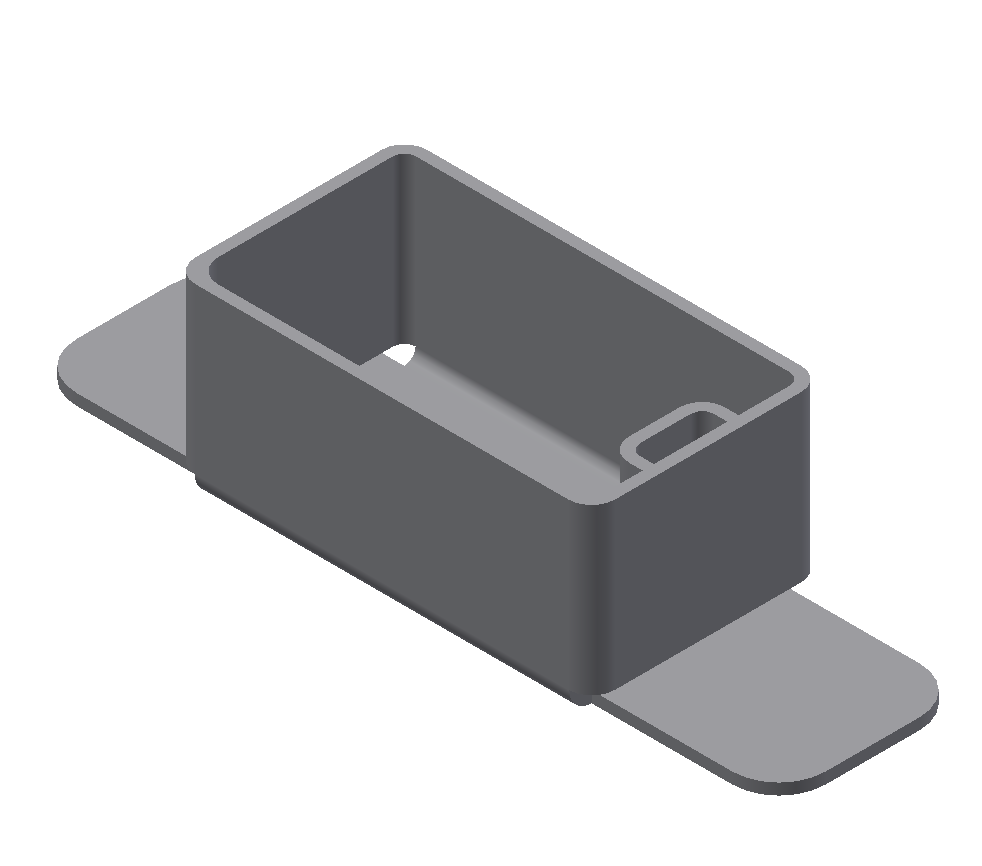
\includegraphics[width=\finalcolumn\linewidth,valign=t]{../Common/images/SheetMetal_Medium_Enclosure_DefeaturedPart}}  
\subfloat[Feature Abstraction]{\label{fig:results:abstraction}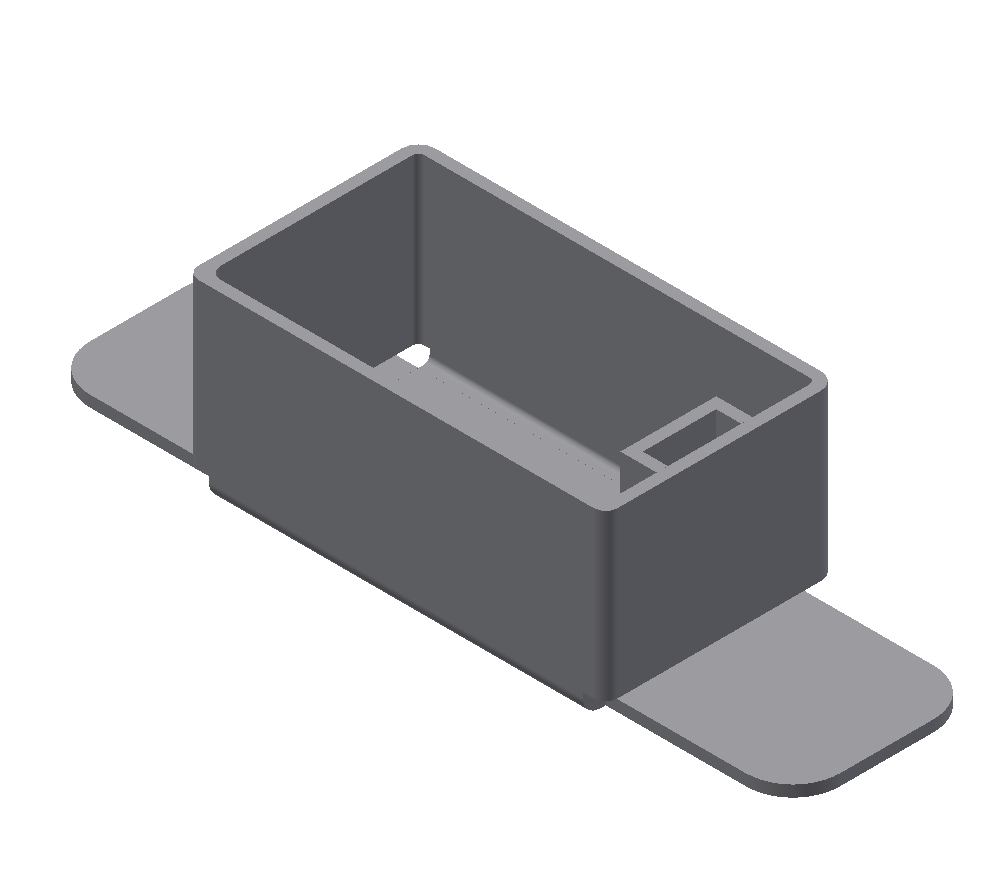
\includegraphics[width=\finalcolumn\linewidth,valign=t]{../Common/images/SheetMetal_Medium_Enclosure_abel_part}} 
\subfloat[Model Decomposition]{\label{fig:results:decomposition}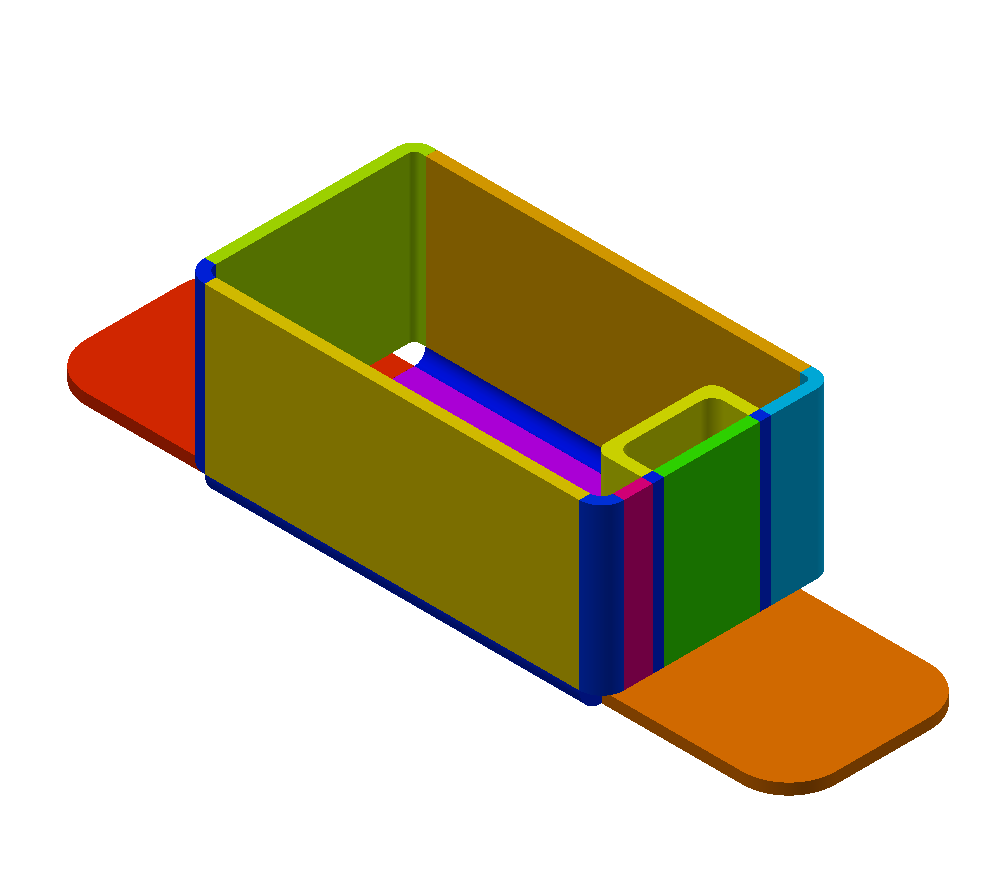
\includegraphics[width=\finalcolumn\linewidth,valign=t]{../Common/images/SheetMetal_Medium_Enclosure_decomp_part}} \\
\subfloat[Midsurface Joining]{\label{fig:results:originalenclosurepart}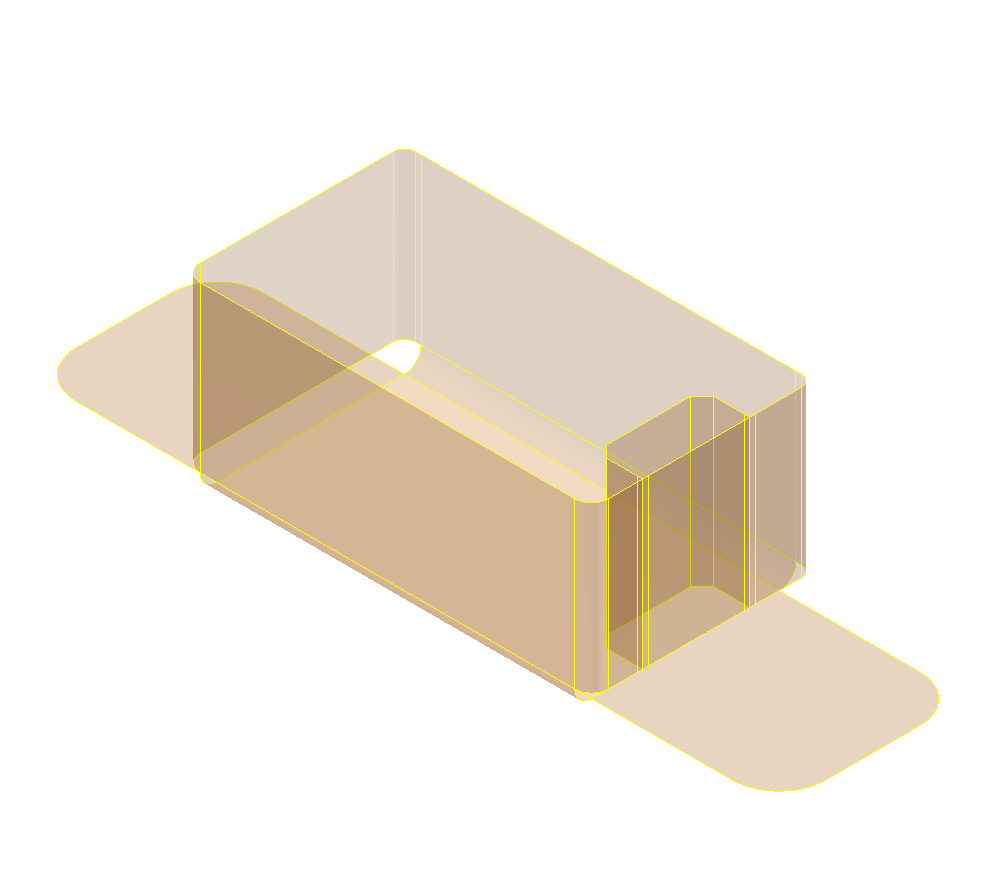
\includegraphics[width=\finalcolumn\linewidth,valign=t]{../Common/images/SheetMetal_Medium_Enclosure_midsurf_part}} 
\subfloat[Dormant Re-application]{\label{fig:results:midsurfbyinventorexnclosure}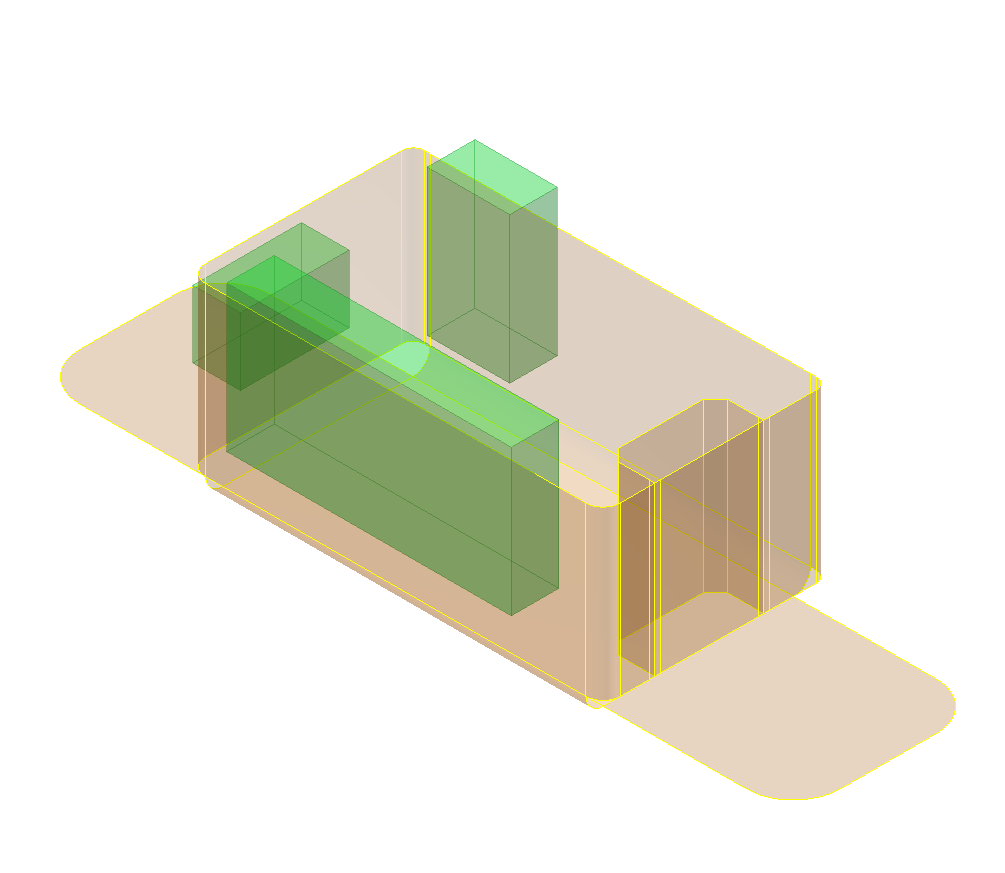
\includegraphics[width=\finalcolumn\linewidth,valign=t]{../Common/images/SheetMetal_Medium_Enclosure_dormant_part}} 
\subfloat[Midsurface Output]{\label{fig:results:mymidsurfenclosure}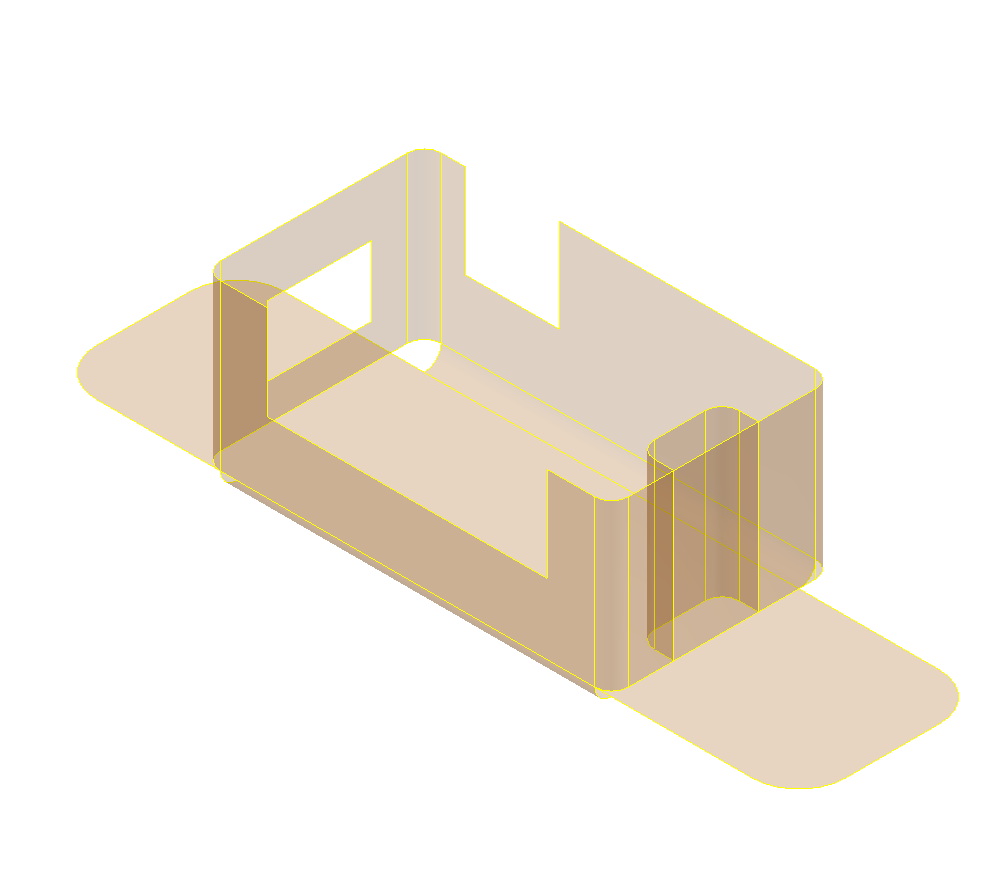
\includegraphics[width=\finalcolumn\linewidth,valign=t]{../Common/images/SheetMetal_Medium_Enclosure_final_midsurf_part}}
\subfloat[Commercial Output]{\label{fig:results:midsurfbyinventorexnclosure}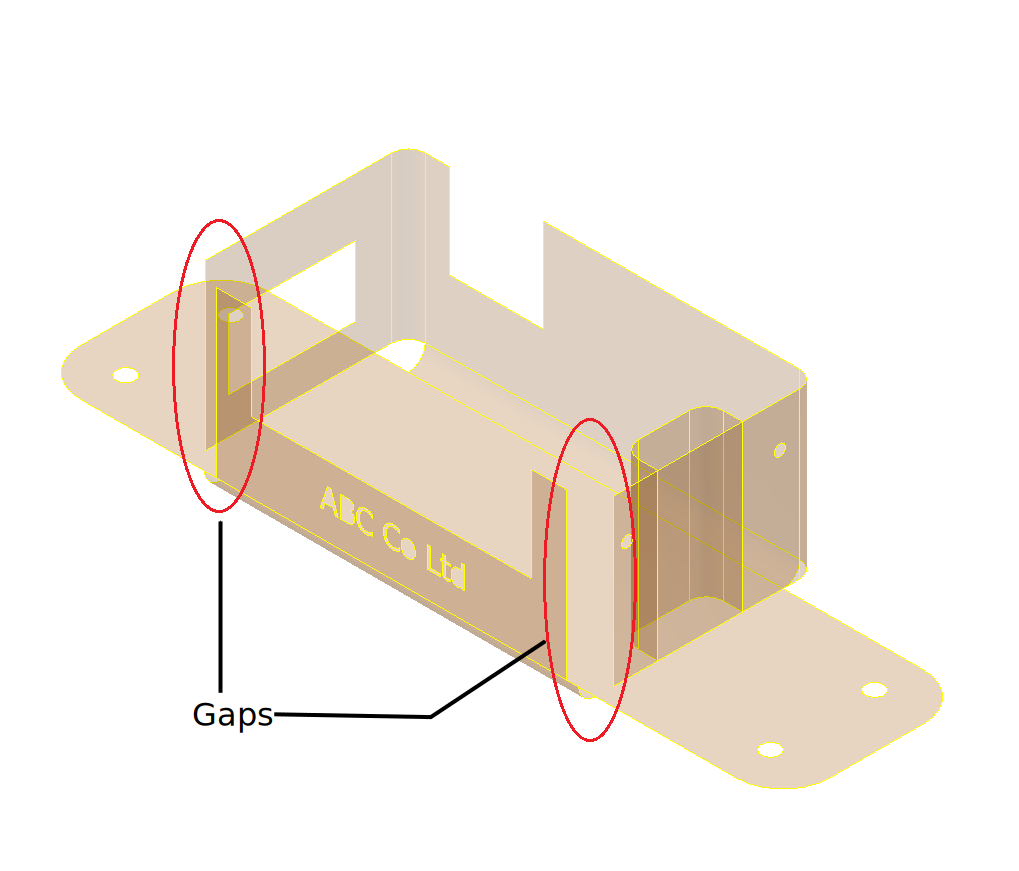
\includegraphics[width=\finalcolumn\linewidth,valign=t]{../Common/images/SheetMetal_Medium_Enclosure_InventorMidsurfwithErrors}}
\caption{Work-flow and Comparison}
\label{fig:results:enlosurebenchmark}
\end{figure}

Figure \ref{fig:results:enlosurebenchmark} show the progress of the algorithm through various modules and last compares with the output from a commercial application. It can be seen that the results from the proposed research are significantly better compared to the commercial application.


Figure \ref{fig:results:stapler} shows one more benchmarking example demonstrating improvements over the commercial output.

\def\onethirdcolumn{0.28}

\begin{figure}[!h]
\centering    
\subfloat[Stapler Model]{\label{fig:results:originalstapler}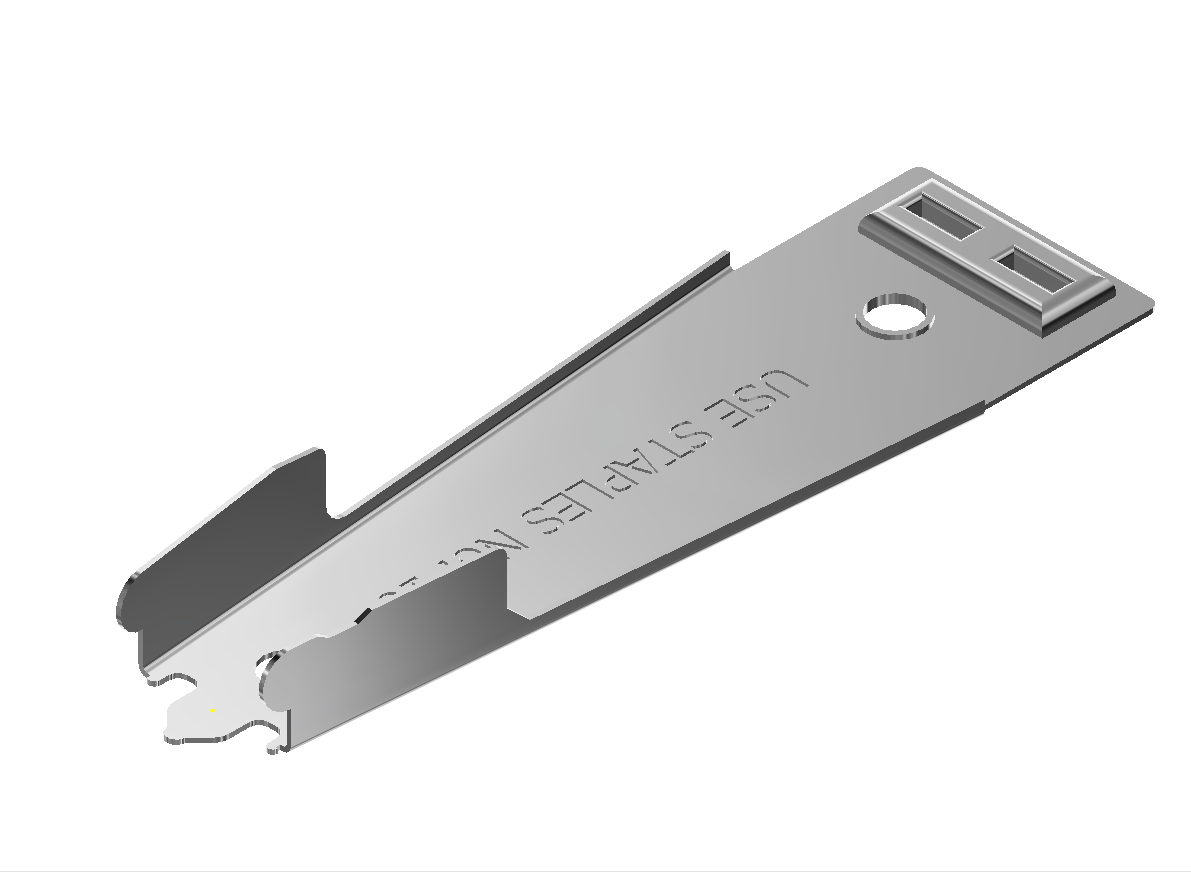
\includegraphics[width=\onethirdcolumn\linewidth,valign=t]{../Common/images/Stapler}} \quad
\subfloat[Commercial Output]{\label{fig:results:hmstapler}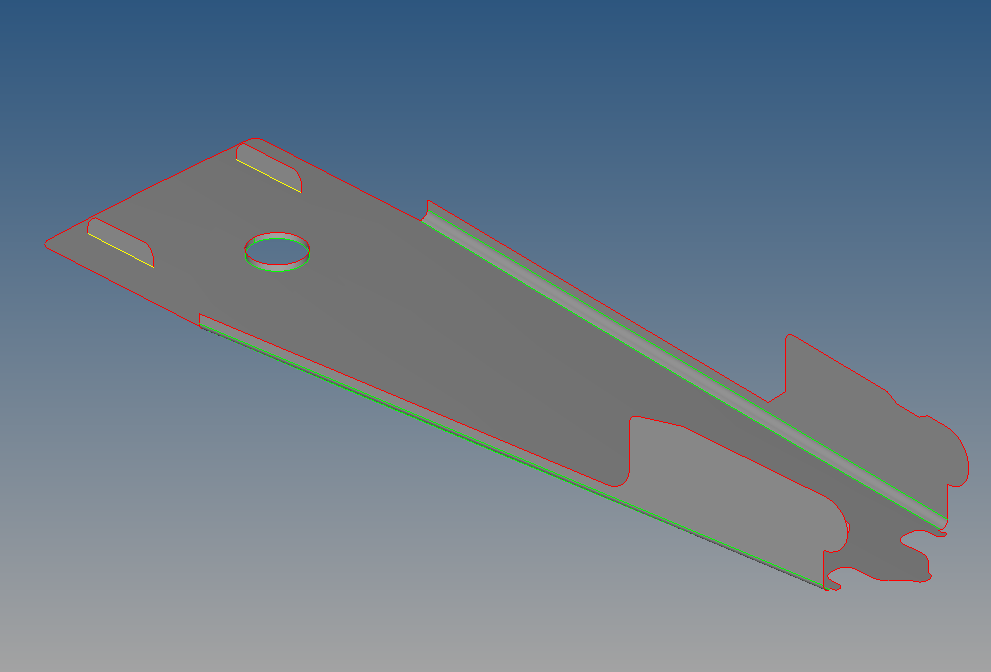
\includegraphics[width=0.3\linewidth,valign=t]{../Common/images/StaplerFails}}  \quad
\subfloat[Research Output]{\label{fig:results:mystapler}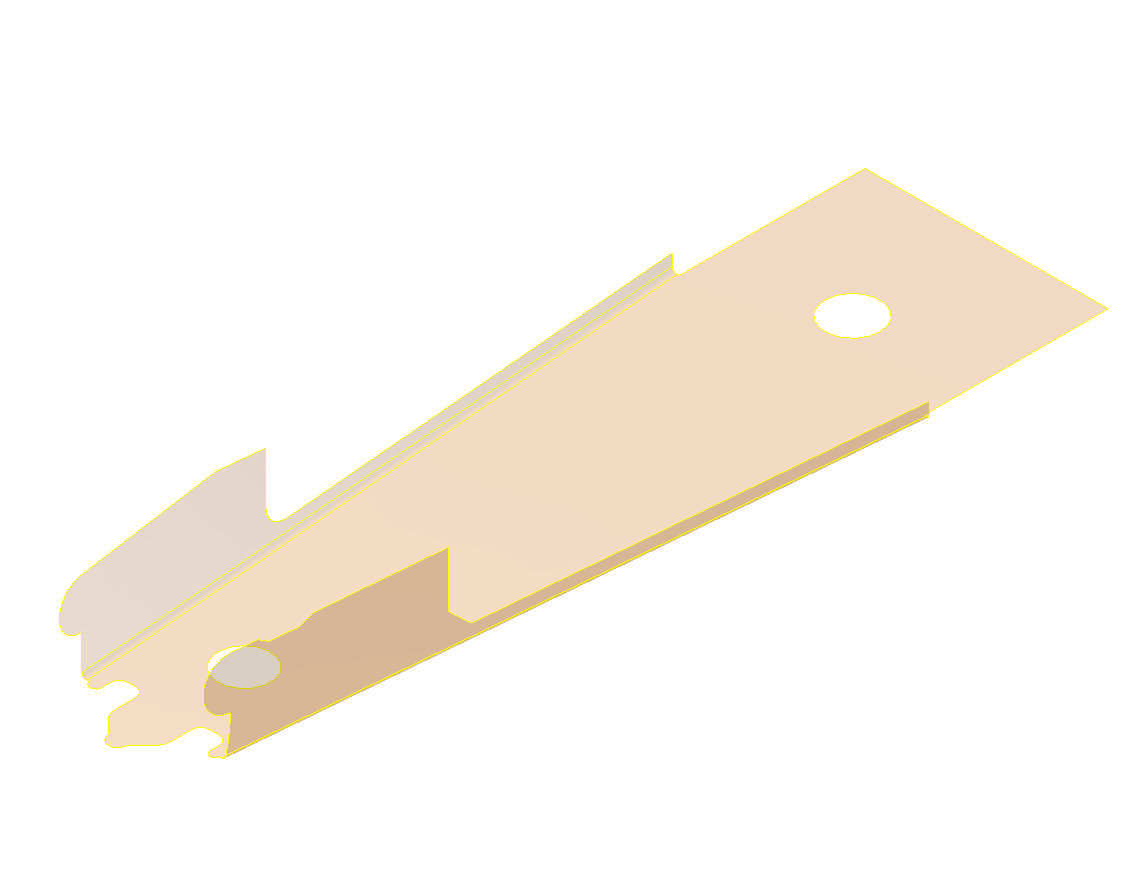
\includegraphics[width=\onethirdcolumn\linewidth,valign=t]{../Common/images/StaplerWorks}} 
\caption{Comparison with Commercial Midsurface Output}
\label{fig:results:stapler}
\end{figure}

Figures \ref{fig:results:bracket} and \ref{fig:results:sbracket} show some additional test-cases to demonstrate the efficacy of the approach.

\def\myfigtestcasescolumnwidth{0.4}
\def\myfigenlosuredefeaturecolumnwidth{0.95}
\def\myfigenlosuredefeatureTreecolumnwidth{0.75}


\begin{figure}[!h]
\centering    
\subfloat[Stapler Model]{\label{fig:results:bracketo}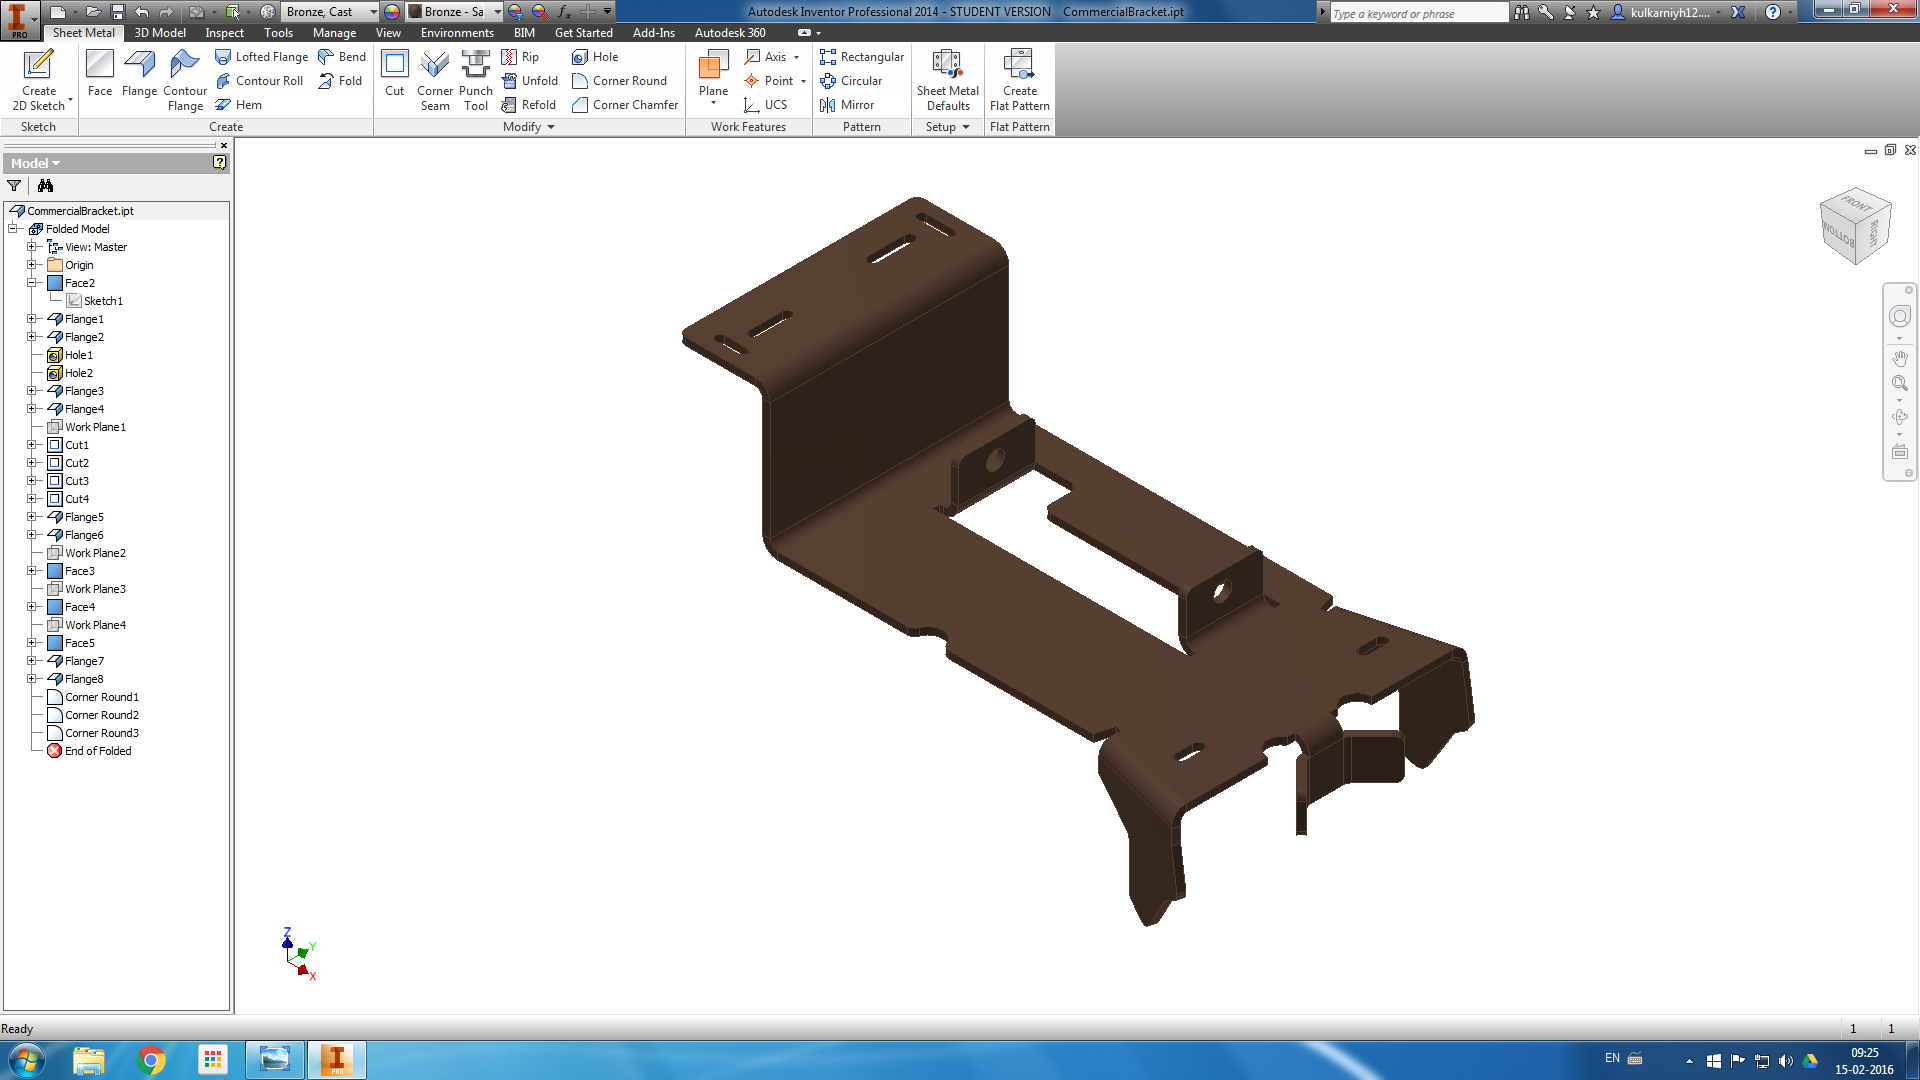
\includegraphics[width=\myfigtestcasescolumnwidth\linewidth,valign=t]{../Common/images/CommercialBracket}} \quad
\subfloat[Research Output]{\label{fig:results:bracketm}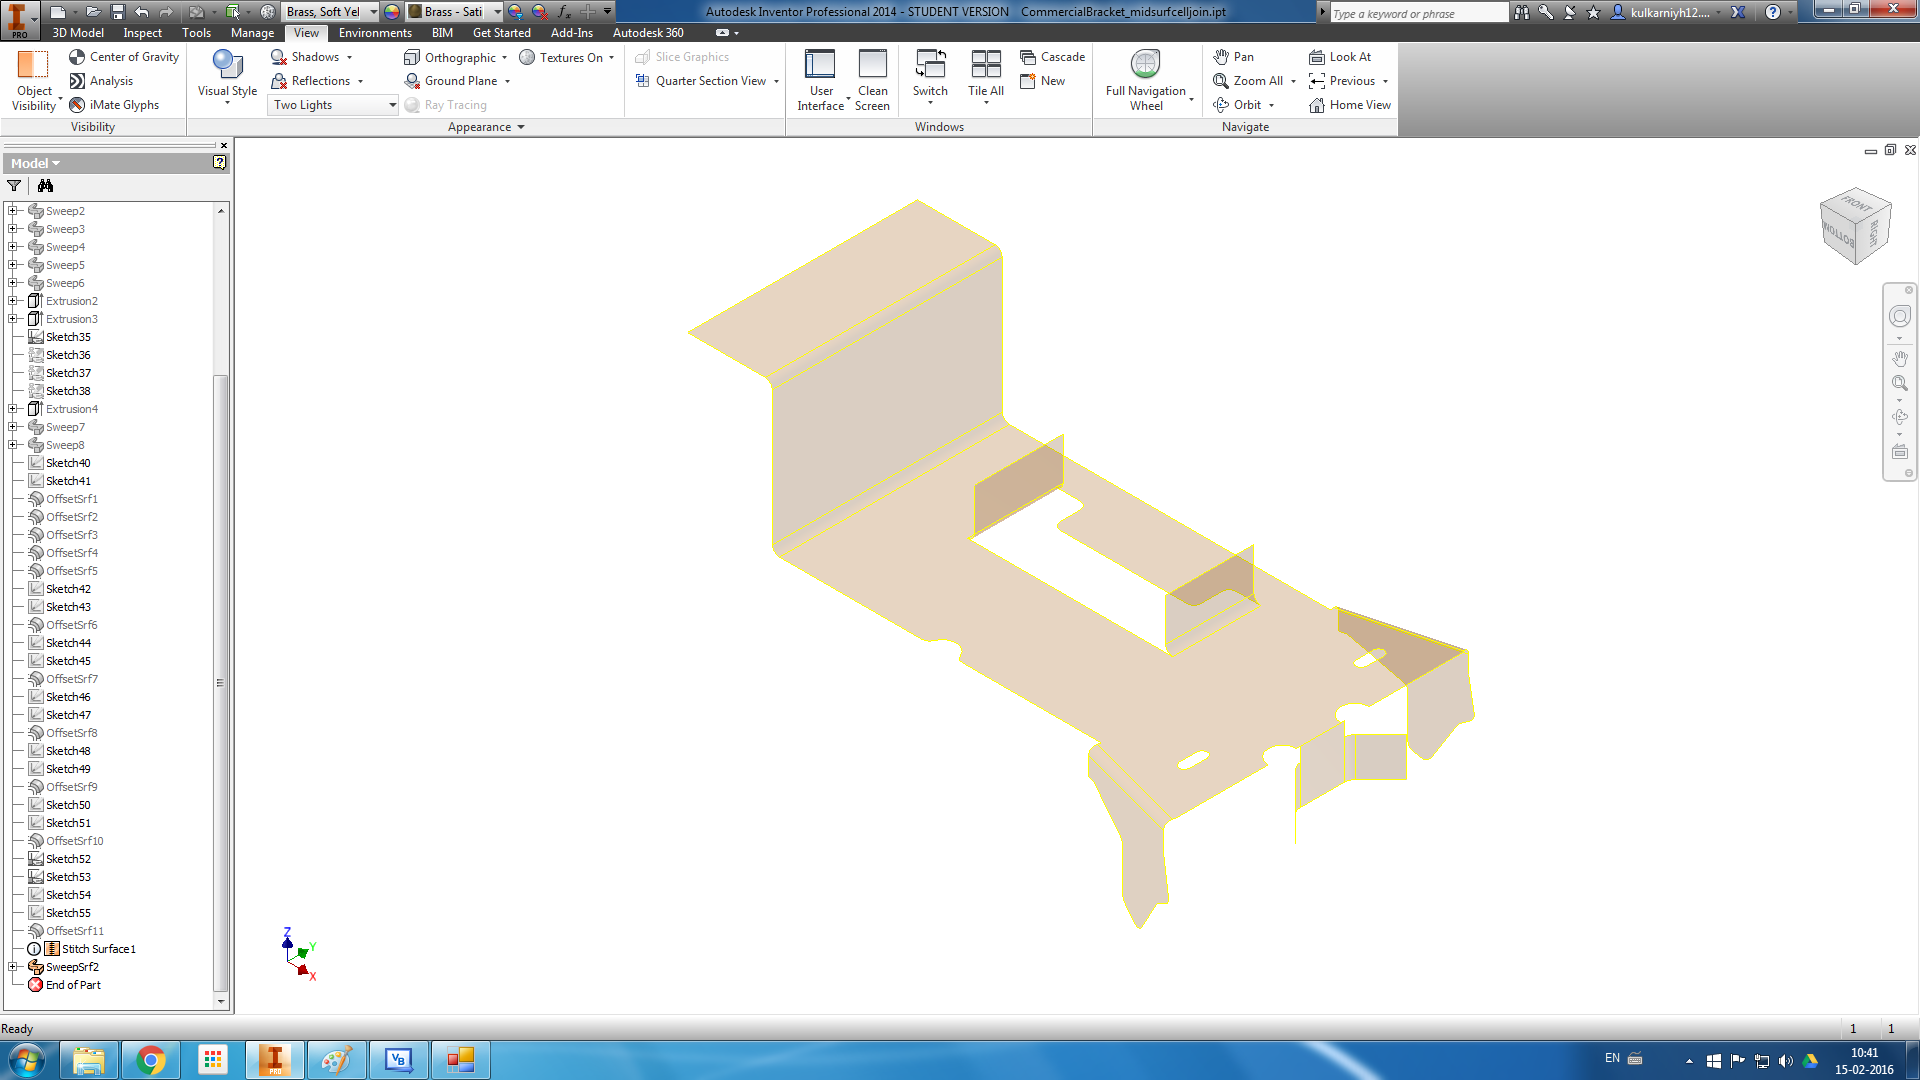
\includegraphics[width=\myfigtestcasescolumnwidth\linewidth,valign=t]{../Common/images/CommercialBracket_midsurfcelljoin}} 
\caption{Input Model and Midsurface Output}
\label{fig:results:bracket}
\end{figure}

\begin{figure}[!h]
\centering  
\subfloat[Bracket Model]{\label{fig:results:sbracketo}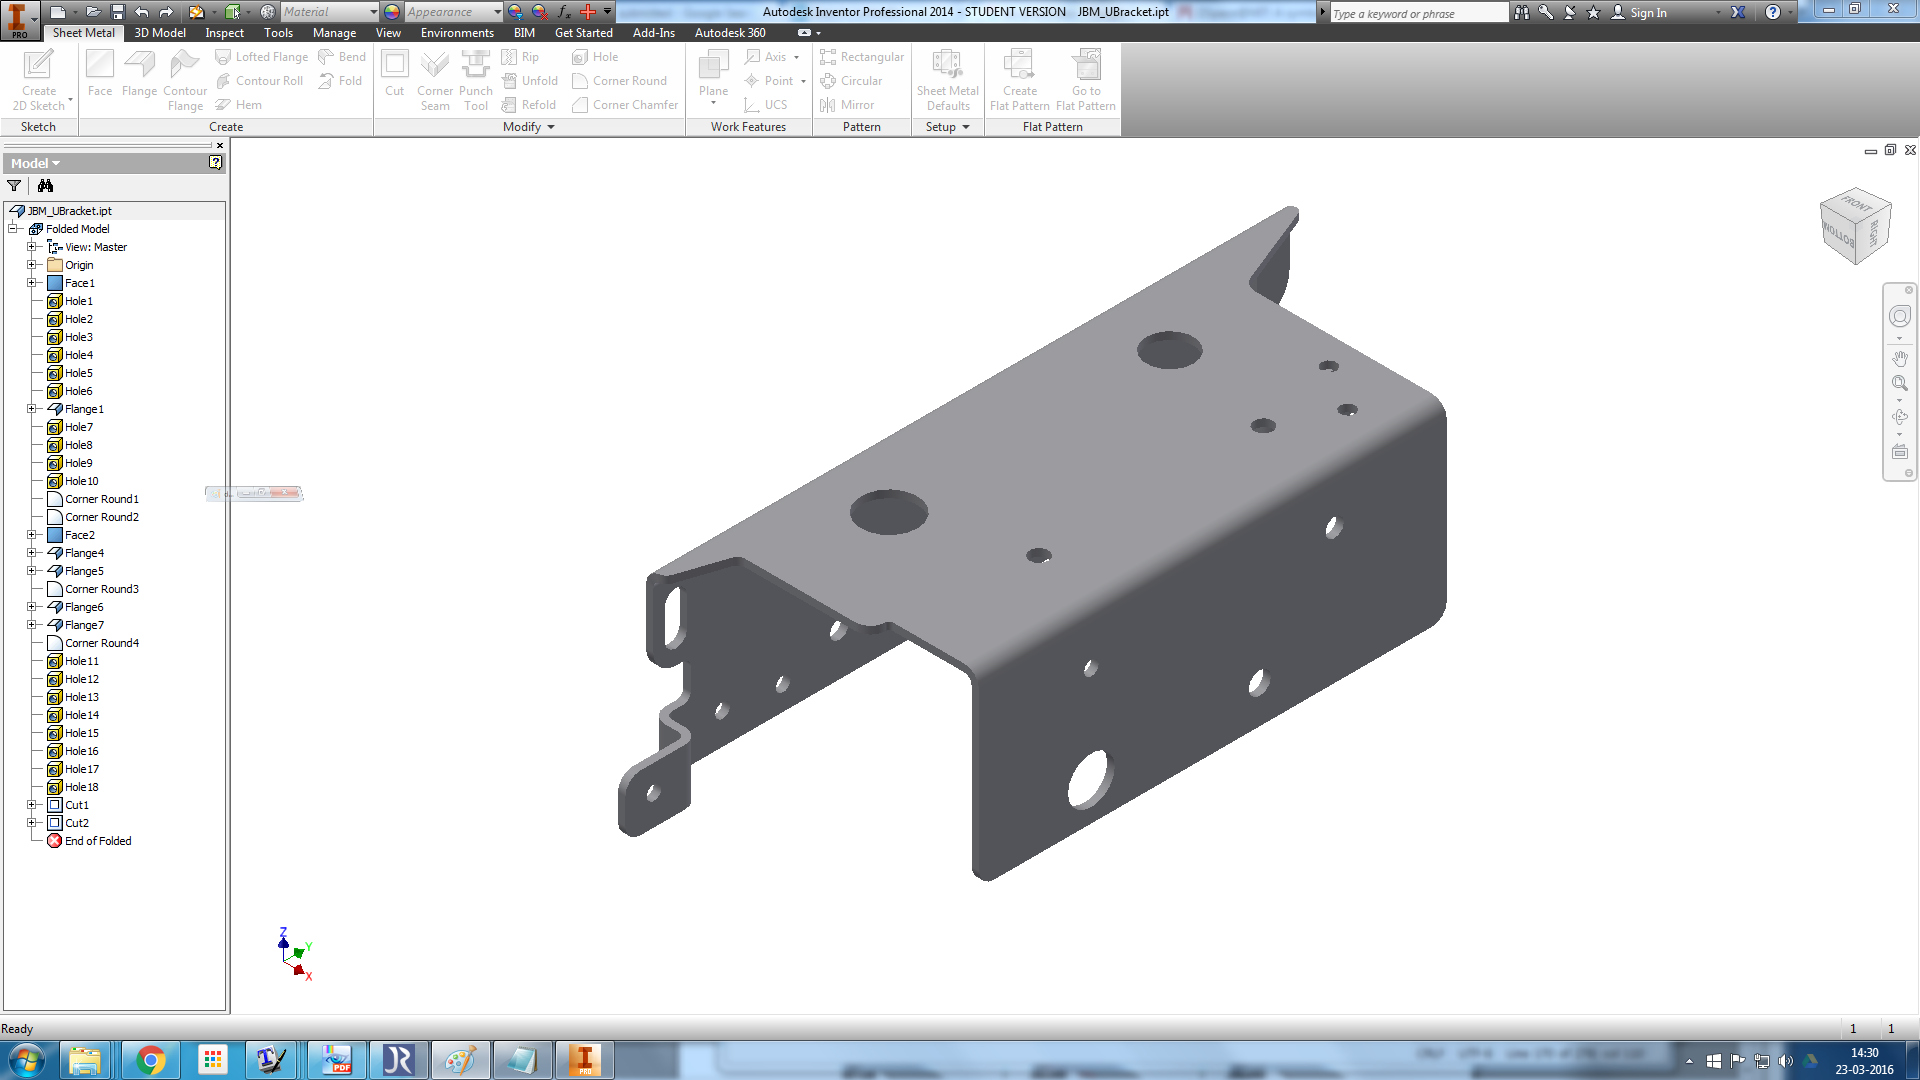
\includegraphics[width=\myfigtestcasescolumnwidth\linewidth,valign=t]{../Common/images/JBM_UBracket_origpart}}  \quad
\subfloat[Research Output]{\label{fig:results:sbracketm}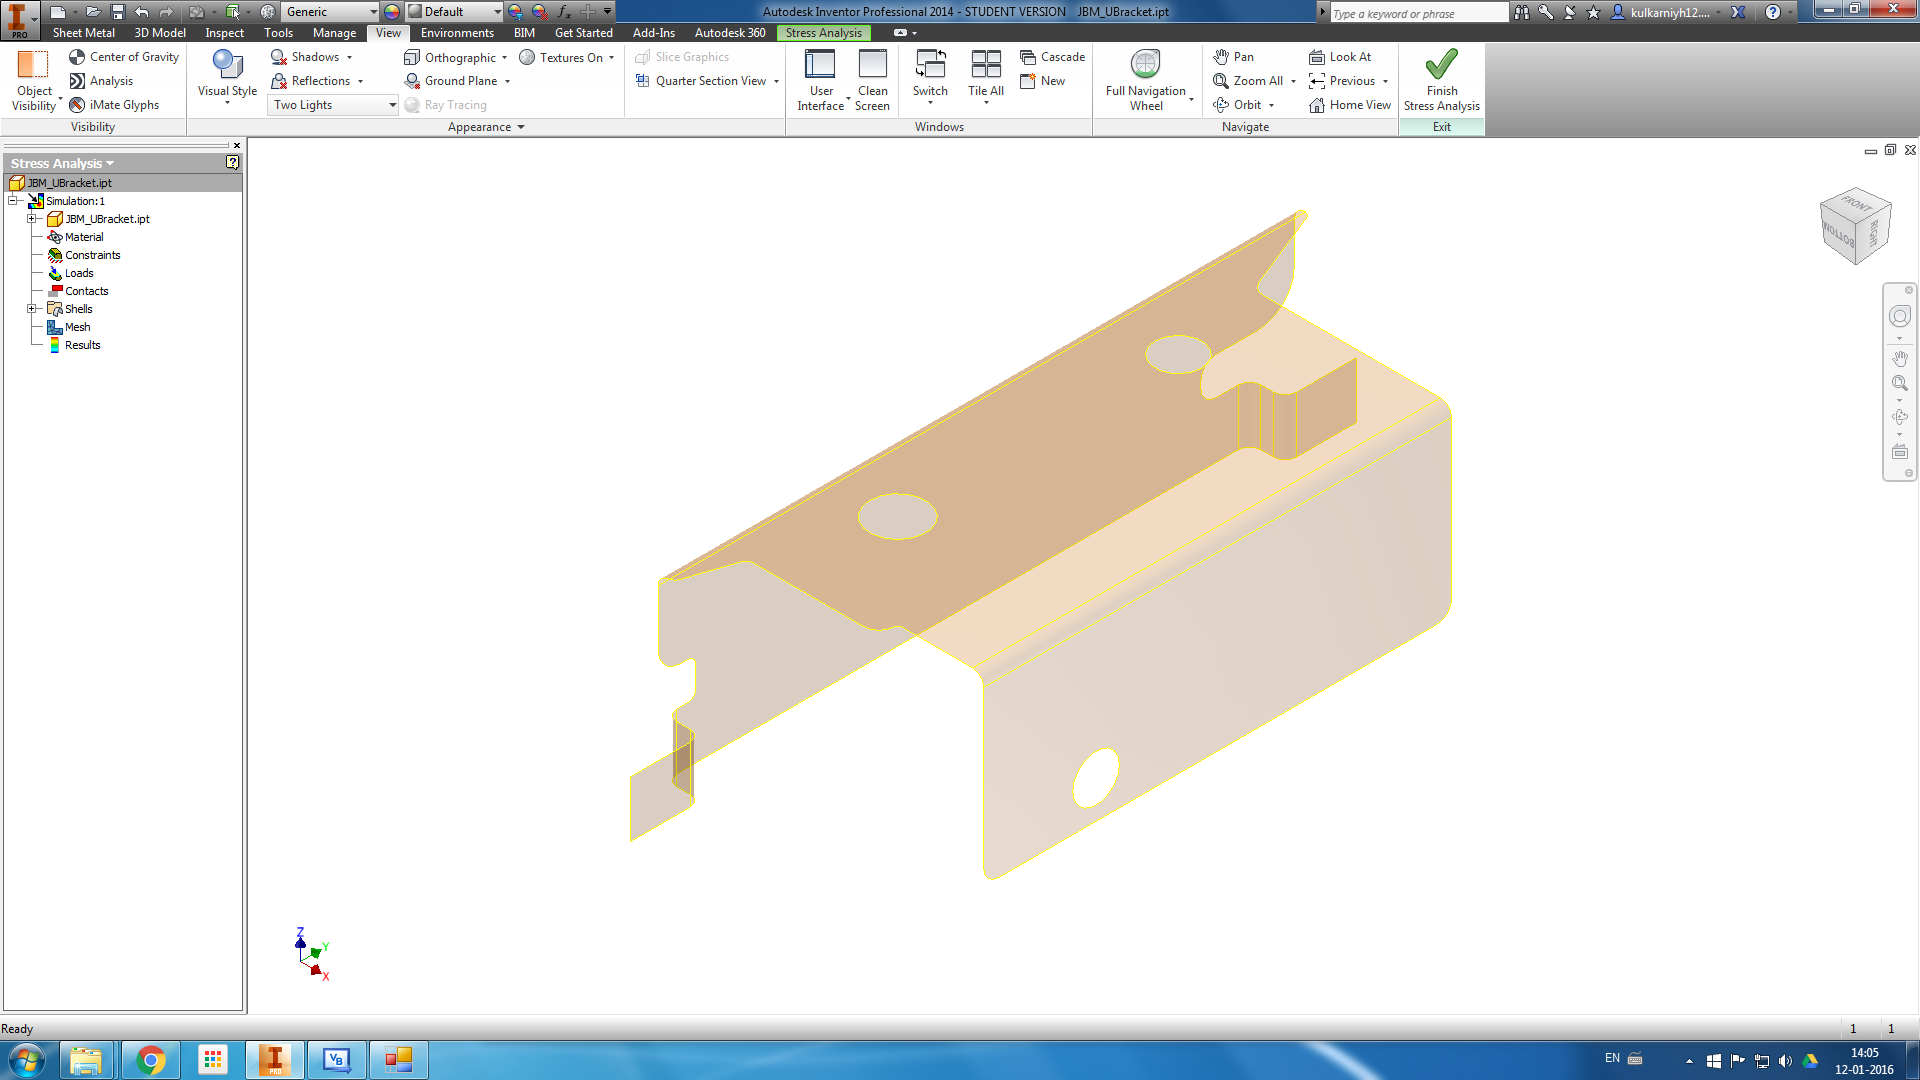
\includegraphics[width=\myfigtestcasescolumnwidth\linewidth,valign=t]{../Common/images/JBM_UBracket_midsurf_after_dormant}} 
\caption{Input Model and Midsurface Output}
\label{fig:results:sbracket}
\end{figure}



